\subsection{Auswahl und Grundlagen der Simulationssoftware}
\label{chap:Auswahl und Grundlagen der Simulationssoftware}

Zur Simulation elektrischer Schaltkreise kann die branchenübliche Software SPICE (Simulation Program with Integrated Circuit Emphasis) zum Einsatz kommen. Auf Basis von SPICE werden von verschiedenen Herstellern Programme entwickelt, welche das Arbeiten durch \zbol ein grafisches Benutzerinterface vereinfachen oder die Software erweitern. Zu diesen Herstellern gehören \ua National Instruments mit ihrem Produkt "`Multisim"' \cite{website:ni:multisim}, Cadence Design Systems mit "`PSpice"' (\cite{website:cadence:pspice}) oder die Analog Devices Inc. mit "`LTSpice"' (\cite{website:analogdevices:ltspice}).

Eine Software, die hier näher betrachtet wird, ist LTSpice. Dieses Produkt zeichnet sich in erster Linie dadurch aus, dass es im Gegensatz zu \zbol Multisim kostenfrei nutzbar ist. Es kommt mit einer umfangreichen Bibliothek an vorgefertigten Makromodellen daher, welche das Konstruieren einer Schaltung vereinfachen und beschleunigen können. LTSpice erlaubt es auch, Schaltungen beliebiger Größe zu simulieren, wobei der limitierende Faktor die Rechenleistung des Systems ist (\cite{Alonso2019}).

Ein Punkt gegen die Nutzung dieser Software ist aber, dass es keine fertigen Implementierungen der Modelle eines analogen Computers in der mitgelieferten Bibliothek gibt. So sind zwar grundlegende Bausteine wie der Operationsverstärker, Widerstände und Kondensatoren vorhanden, aber Modelle wie eine Gilbert Zelle zum Multiplizieren oder ein Funktionsgenerator fehlen. Auch öffentlich zugängliche externe Bibliotheken bieten nicht den für diese Arbeit geforderten Umfang an Modellen (\cite[vgl.]{website:github:ltspice-analog-computer}). Die Entwicklung einer geeigneten Bibliothek passt nicht in den Umfang dieser Arbeit und erfordert zusätzlich ein nicht vorhandenes Maß an Vorwissen im Bereich Elektrotechnik. Aufgrund dessen eignet sich LTSpice nicht für den Einsatz in dieser Arbeit.

Als Erweiterung zu Matlab kommt Simulink für diese Arbeit infrage, eine grafische Entwicklungsumgebung für modellbasierte Systementwicklung. Simulink zeichnet sich durch die Modellierung von Programmen durch Blockdiagramme aus und stellt Funktionen zur Simulation und Analyse bereit. Des Weiteren lässt sich Source-Code für \zb C++ aus den Programmen generieren. Ein Modell in Simulink besteht aus Blöcken, Signalen und Kommentaren. Blöcke stellen mathematische Funktionen bereit, Signale verbinden diese Blöcke und können verschiedene Datentypen wie Skalare, Vektoren oder Matrizen darstellen. Kommentare erlauben das beliebige Einfügen von Text und Bildern in die grafische Oberfläche (\cite{Peasley2018}).

Die von Simulink vorgegebenen Blöcke sind in Bibliotheken aufgeteilt. In "`Sources"' befinden sich diverse Blöcke wie Konstanten, Sinus-Kurven oder Puls-Generatoren zur Eingabe in das Modell. "`Sinks"' bietet Blöcke zur Darstellung oder dem Export von Signalen, wie dem "`Scope"' zur Darstellung eines Graphen oder "`Display"' zur einfachen Anzeige von Werten, an. Auch alle für diese Arbeit relevanten mathematischen Operationen sind in Simulink innerhalb der Bibliothek "`Math Operations"' vorhanden. Dazu zählen Funktionen wie Summierung, Multiplizierung und Koeffizienten. Die Bibliothek "`Continuous"' beinhaltet Funktionen speziell für kontinuierliche Signale, wie sie in analogen Rechner genutzt werden. Dazu zählen primär die Integration bzw. die Ableitung eines Signals. Unter "`Discrete"' befinden sich demnach Blöcke für diskrete Signale, die in dieser Arbeit aber nicht zum Einsatz kommen können. Letztlich bietet Simulink eine nützliche Funktion zur Vereinfachung und Validierung von Modellen mit den "`User Defined Functions"' an, womit Matlab-Code einfach in ein Simulink-Modell integriert werden kann. (\cite[vgl.]{Peasley2018})

Wie mithilfe der genannten Blöcke das Masse-Pfeder-Dämpfer System aus Abbildung \ref{fig:Feder-Masse-D\"ampfer System mit R\"uckkopplung} modelliert werden kann, wurde bereits von \citeauthor{Ulmann2022} gezeigt:

\begin{figure}[h]
  \caption{Simulation eines Masse-Feder-Dämpfer Systems in Simulink}
  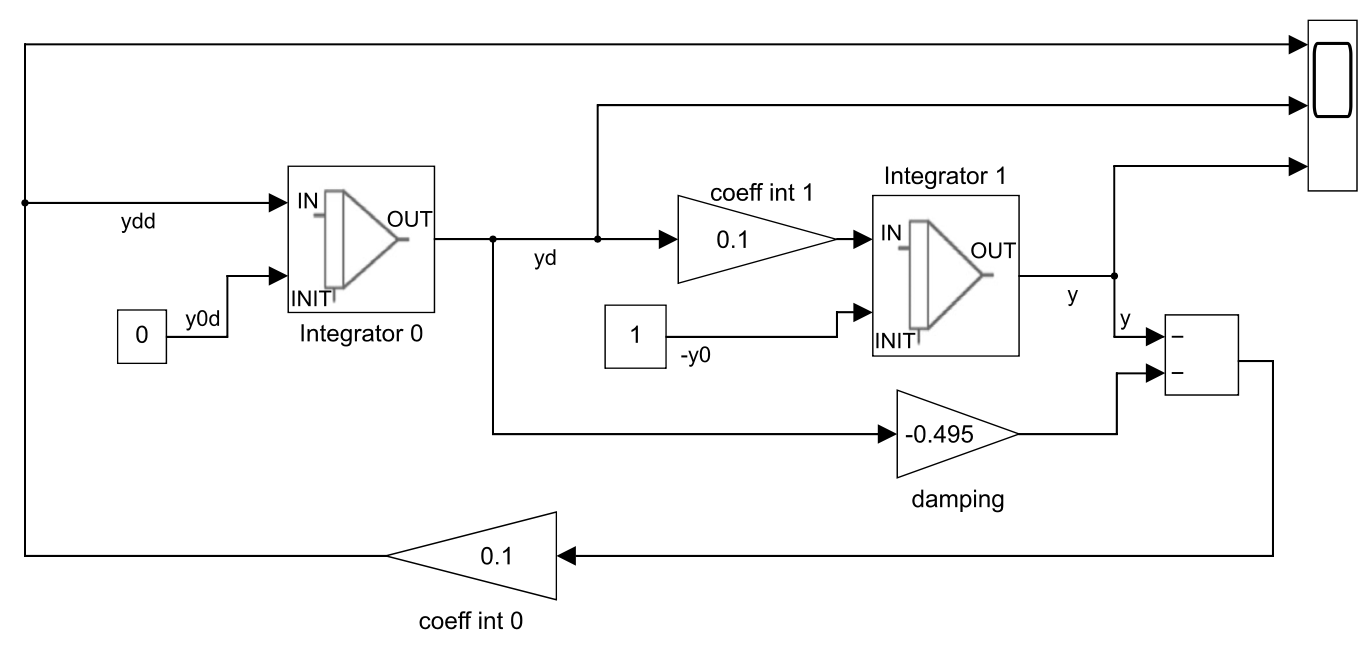
\includegraphics[width=\textwidth]{abbildungen/simulink_beispiel.png}
  \\
  Quelle: \cite[S. 241]{Ulmann2022}
  \label{fig:Masse-Feder-Dämpfer Simulink}
\end{figure}

Zusätzlich zur Standard-Bibliothek lässt sich Simulink durch weitere Produkte erweitern. Zur Modellierung physikalischer Systeme wird \zb "`Simscape"' angeboten, womit Simulink um die Simulation mechanischer, elektrischer, hydraulischer und thermaler Systeme erweitert wird. Durch die Installation dieser Erweiterung werden auch Komponenten der Elektrotechnik wie der Operationsverstärker, Widerstand oder Kondensator zur Bibliothek hinzugefügt, wodurch analoge Rechenelemente modelliert werden können. Eine Implementierung des Masse-Feder-Dämpfer Systems anhand dieser Komponenten ist in Abbildung \ref{fig:Simulink und Simscape} dargestellt. Physikalische Signale können mit den herkömmlichen Simulink-Blöcken über Signal-Konverter verbunden werden, wodurch Simulink- und Simscape-Modelle miteinander kompatibel werden (\cite{website:mathworks:simscape}). Für diese Arbeit wird jedoch nur Simulink betrachtet, die theoretischen Konzepte werden also nicht physikalisch modelliert.

\begin{figure}[h]
  \caption{Masse-Feder-Dämpfer System in Simulink und Simscape}
  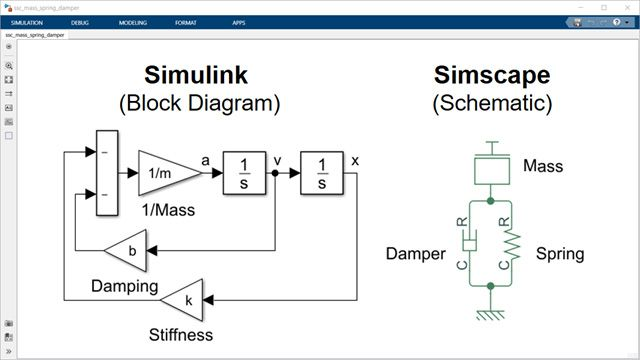
\includegraphics[width=\textwidth]{abbildungen/simulink_simscape.jpg}
  \\
  Quelle: \cite{MathWorksSimscape}
  \label{fig:Simulink und Simscape}
\end{figure}
